\subsection*{Ejercicio 5}

\ejercicio{Considere ahora la situación del mejor caso posible en la
  que el vector de entrada ya está ordenado. ¿Cuál sería la eficiencia
  teórica en ese mejor caso? Muestre la gráfica con la eficiencia
  empírica y compruebe si se ajusta a la previsión.}

\begin{flushleft}
  El caso en el cual todos los elementos del vector estan ordenados el
  programa solo realiza operaciones elementales (comparaciones y
  operaciones) n veces, luego la complejitud del problema será lineal, $O(n)$.

  \begin{figure}[H]
  \centering
    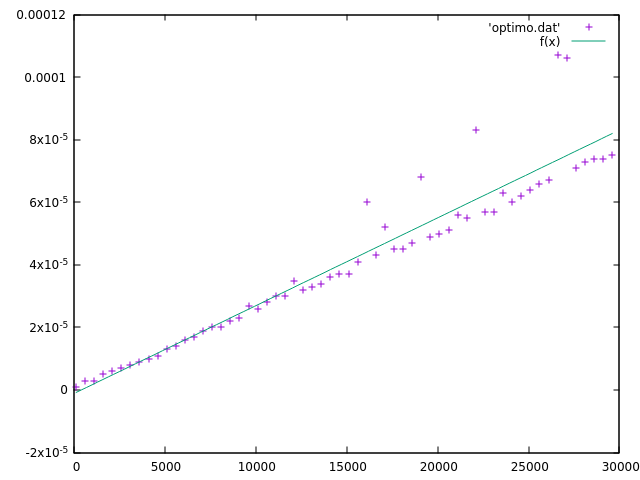
\includegraphics[width=0.7\textwidth]{ejer5/resultado.png}
  \end{figure}
  
\end{flushleft}
